\chapter{Reproduktion bisheriger Ergebnisse}
\label{chap:reproduktion}
\epigraph{What I cannot create, I do not understand}{--- Richard Feyman}

\section{Datensatz}

\section{Auswahl und Beschreibung des Datensatzes}
\textcite[985\psqq]{DoermannHandbookdocumentimage2014} listen 5 Aspekte die bei der Erstellung von Datensätzen zu beachten sind:
\begin{itemize}
    \item Auswahl der Daten
    \item Datenbeschaffung
    \item Ground Truth Definition
    \item Ground Trouth Annotation
    \item Speicherformat
    \item Struktur und Organisation
\end{itemize}

\section{DIVA-HisDB}
Die DIVA \marginnote{\url{http://diuf.unifr.ch/main/diva/}} (Document, Image and Voice Analysis) Gruppe der Universität Fribourg hat im Kontext der Forschungsprojekte HisDoc und HisDoc 2.0 
das Datenset DIVA-HisDB. erstellt.
Die HisDoc-Projekte beschäftigen sich mit der automatischen Analyse von historischen Dokumenten und
wie man diese für Historiker nutzbar machen kann.

\cite{SimistiraDIVAHisDBPreciselyAnnotated2016}

% Auswahl der Daten
Für den Datensatz wurden Dokumente mit komplexen Layout aus der Virtuellen Manuskriptbibliothek der Schweiz (\url{http://www.e-codices.unifr.ch/en}) ausgesucht. 
\research{Manuskriptbibliothek}

% Struktur und Organisation 
Die Manuskripte enthalten neben dem Haupttext auch Randnotizen und Text-Dekorationen. 
Randnotizen befinden sich auch teilweise zwischen den Zeilen des Haupttexts.
DIVA-HisDB besteht aus 150 Dokumenten, aufgeteilt in Trainings-, Validierungs- und Testset (siehe \cref{table:hisdb_pages}. 
Hinzu kommen 30 Seiten die für die finale Wertung des Wettbewerbs ``ICDAR2017 Competition on Layout Analysis for Challenging Medieval Manuscripts'' verwendet wurden.

\begin{table}
    \caption{Aufteilung der Seiten des DIVA-HisDB-Datenssets}
    \label{table:hisdb_pages}
    \begin{tabular}{lccccc}
        {\bfseries Name} & {\bfseries Auflösung} & {\bfseries Training} & {\bfseries Validierung} & {\bfseries Test} & {\bfseries Test ICDAR 2017)}\\
        \csvreader[head to column names]{tables/diva_hisdb_specs.csv}{}%
        {\name&	\width \(\times\)\height & \train	&\validate	&\test	&\comp\\}
    \end{tabular}
\end{table}

% Datenbeschaffung
Alle Daten können direkt von der Webseite der DIVA-Gruppe heruntergeladen werden.

% Speicherformat
Die Manuskripte wurden mit einer Auflösung von 600 dpi gescannt und sind im  JPEG-Format gespeichert. 
Die \cref{table:hisdbsamples} zeigt Beispiele aus den drei Datensätzen. 

% Ground Truth Definition
Der Datensatz wurde semi-automatisch mit 3 Annotation (Haupttext, Kommentare, Dekorationen) versehen.
Alle Bereiche die nicht annotiert sind werden als Bildhintergrund betrachtet.

% Ground Trouth Annotation
Diese Ground-Truth-Annotationen sind im PAGE-XML-Format und als ``pixel-label'' PNG-Bilder gespeichert.
Die \cref{fig:ground_truth} zeigt eine Beispielseite mit den zugehörgine Labels auf Pixelebene. 

\begin{figure*}
    \centering
    \caption{Hintergrund: weiss, Haupttext: blau, Kommentare: grün, Dekorationen: rot }
    \label{fig:ground_truth}
    \subfloat[Dokumentenbild]{%
        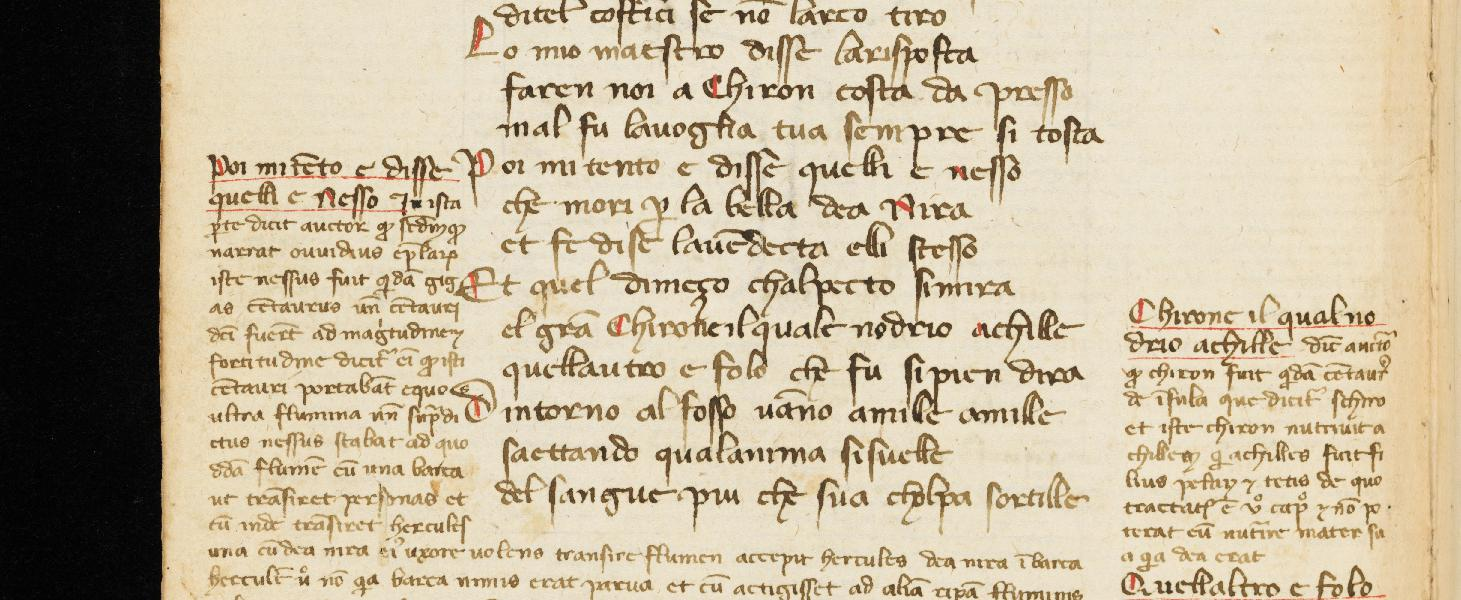
\includegraphics[width=0.5\textwidth]{figures/datasets/gt_example0.jpeg}
    }
    \subfloat[``pixel-label'']{%
        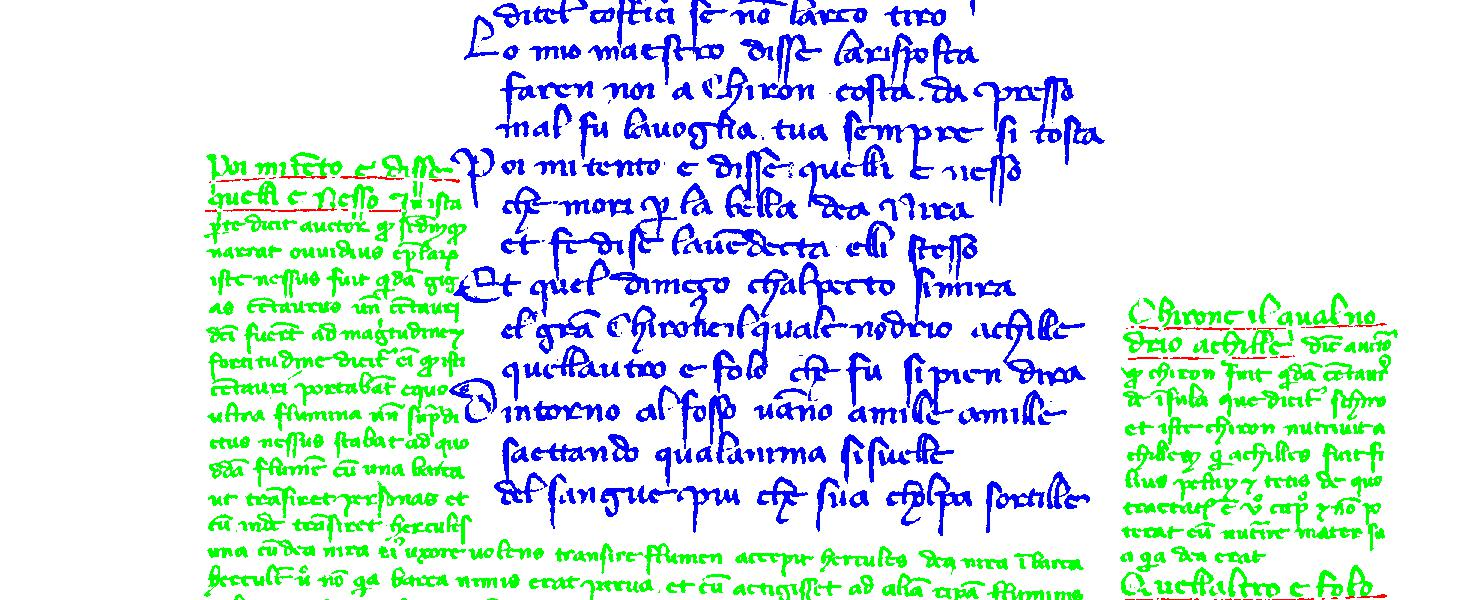
\includegraphics[width=0.5\textwidth]{figures/datasets/gt_example1.jpeg}
    }
\end{figure*}

Die Menge an Pixeln pro Klasse ist sehr unterschiedlich.
Die \cref{table:class_distribution} zeigt das in jedem Dokumentenset der Hintergrund deutlich überwiegt.

\begin{table}
    \caption{Verteilung der Klassen in Prozent\autocite[1362]{SimistiraICDAR2017CompetitionLayout2017}}
    \label{table:class_distribution}
    \begin{tabular}{lrrrr}
        {\bfseries Set} & {\bfseries Hintergrund} & {\bfseries Kommentar} & {\bfseries Dekoration} & {\bfseries Text}\\
        \csvreader[head to column names]{tables/diva_hisdb_class_distribution.csv}{}%
        {\set&	\background & \comments & \decoration & \text \\}
    \end{tabular}
\end{table}



\begin{table*}
    \begin{tabular}{llp{4cm}}
        \vspace{0.2cm}
        {\bfseries Seite} & {\bfseries Detailauschnitt} & {\bfseries Quelle } \\
        \vspace{0.5cm}
        
        \raisebox{-.5\height}{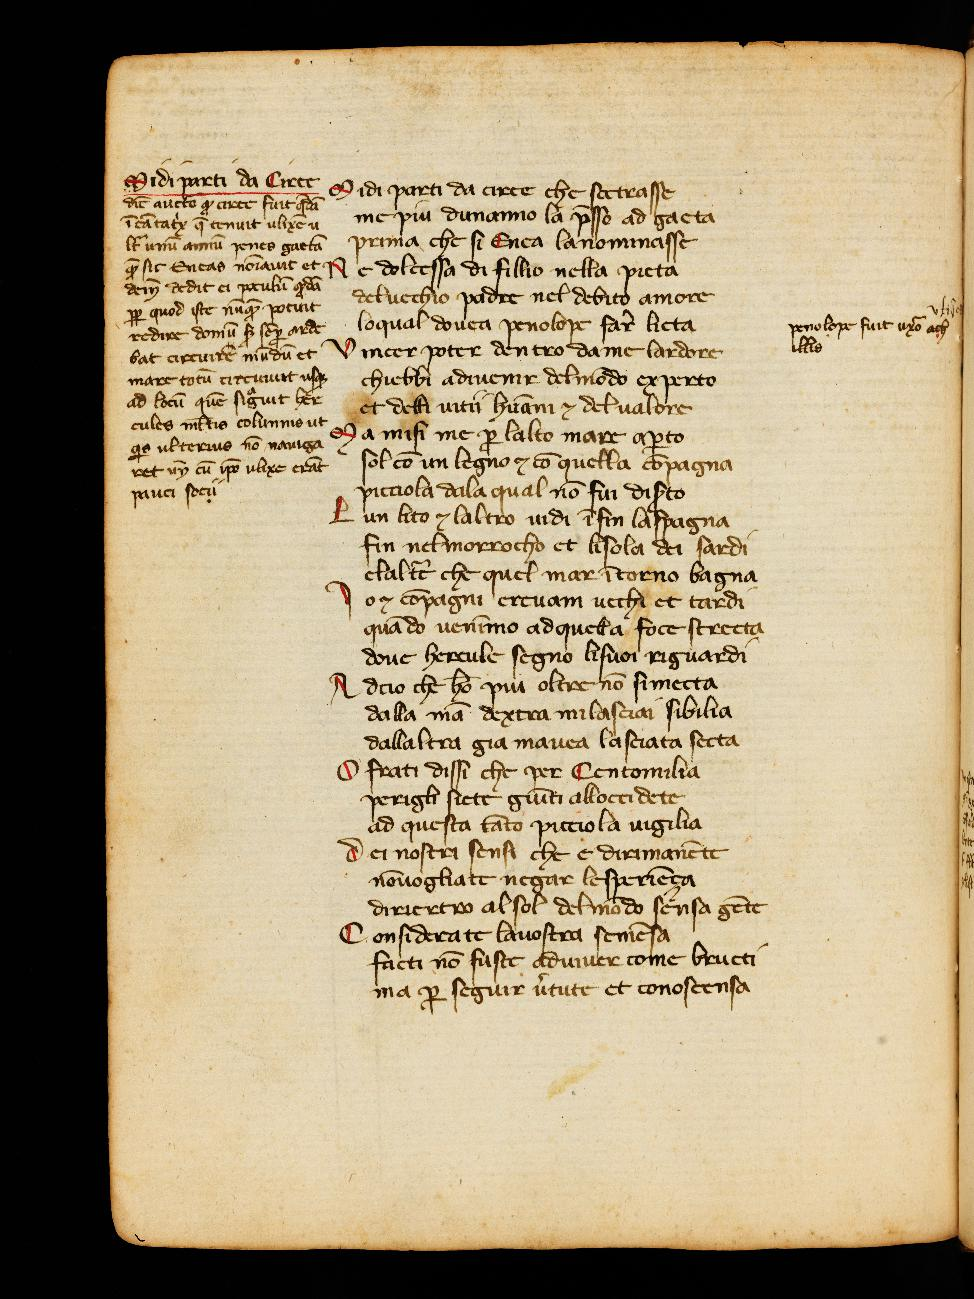
\includegraphics[height=4cm]{figures/datasets/HisDBSample0.jpeg}}
    &\raisebox{-.5\height}{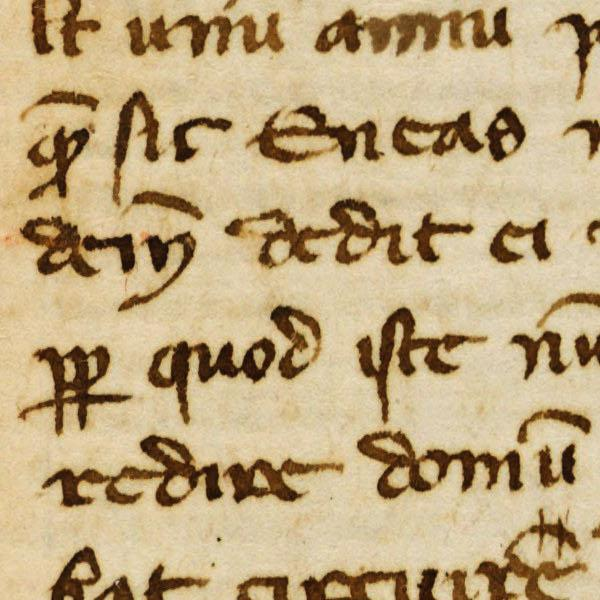
\includegraphics[height=4cm]{figures/datasets/HisDBSampleBox0.jpeg}}
     & \citefield{AlighieriColognyFondationMartin1300}{title}\\
     \vspace{0.5cm}  
     
    \raisebox{-.5\height}{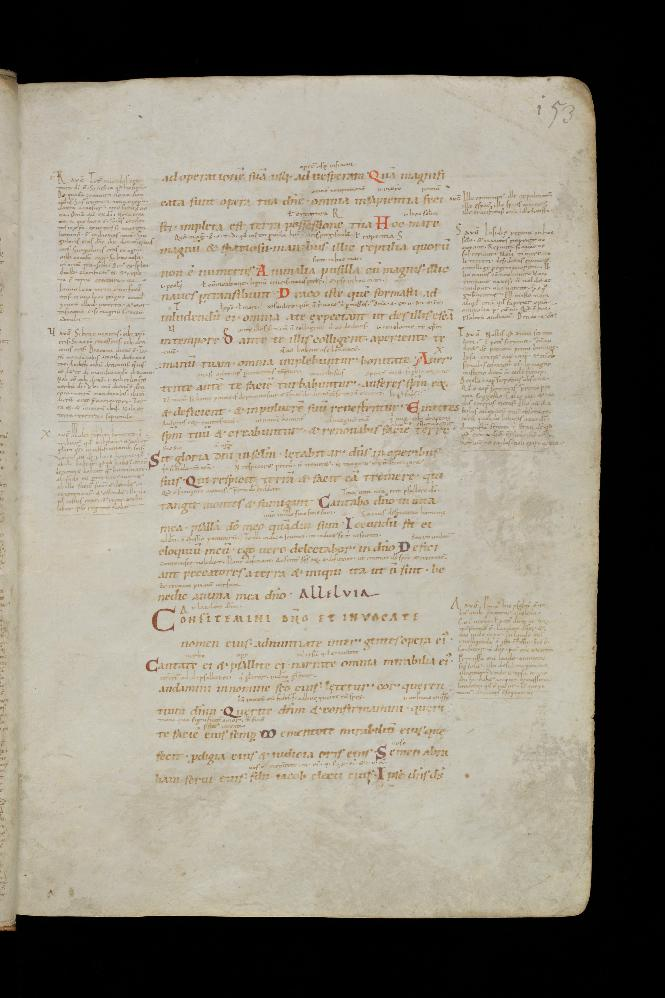
\includegraphics[height=4cm]{figures/datasets/HisDBSample2.jpeg}}
    & \raisebox{-.5\height}{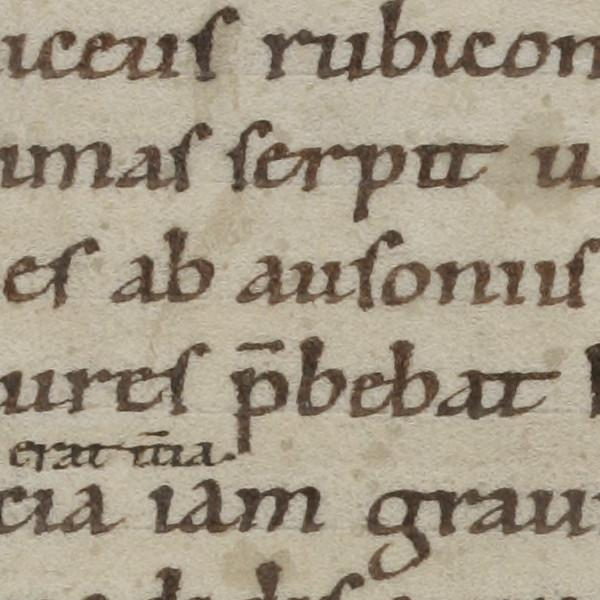
\includegraphics[height=4cm]{figures/datasets/HisDBSampleBox2.jpeg}}
    & \citefield{AmbrosiusStGallenStiftsbibliothek985}{title}\\
    \vspace{0.5cm}
    
     \raisebox{-.5\height}{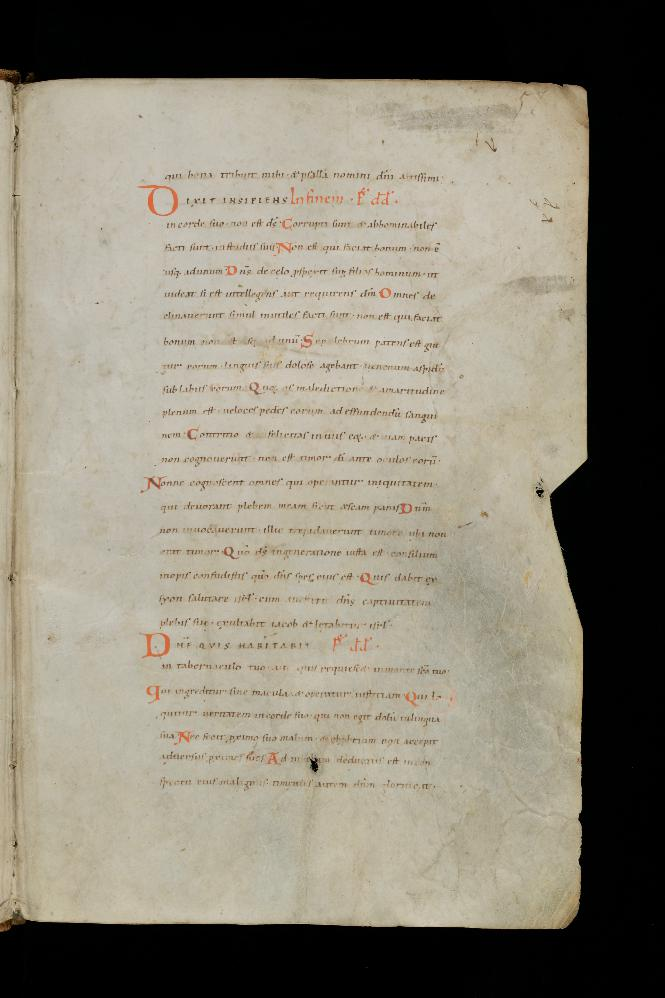
\includegraphics[height=4cm]{figures/datasets/HisDBSample1.jpeg}}
    &\raisebox{-.5\height}{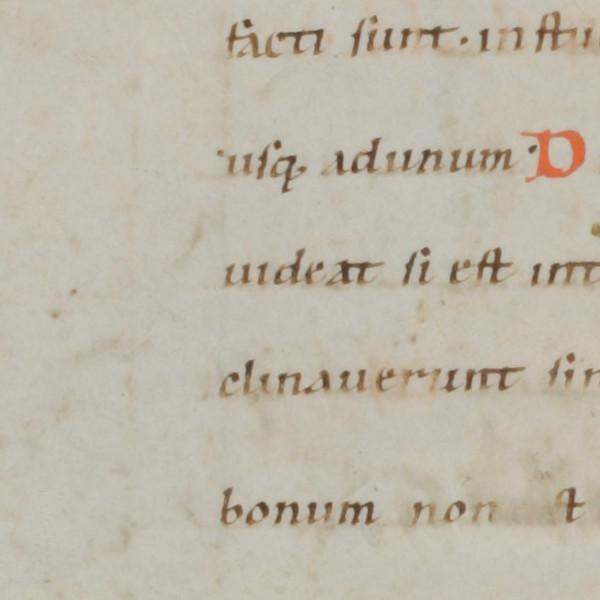
\includegraphics[height=4cm]{figures/datasets/HisDBSampleBox1.jpeg}}
     & \citefield{LucanusStGallenStiftsbibliothek1025}{title}\\
     \vspace{0.5cm} 

    \end{tabular}
    \caption{HisDB Beipsiele mit Detailauschnitt}
    \label{table:hisdbsamples}
\end{table*}



\qq{welche Experimente?}
Im folgenden werden Paper genauer untersucht, die sich mit dem Problem der Dokumentensegmentierung mit Hilfe von CNNs nähern.
Das erste Experiment basiert auf dem neusten Paper von Mitgliedern der DIVA-Gruppe: \citeauthor*{ChenConvolutionalNeuralNetworks2017}. 

Das zweite Experiment basiert auf der Forschung des Gewinners des IDCAR2017-Wettbewerbs: \citeauthor*{XuPageSegmentationHistorical2017} 

\section{Andere Ansätze}
\cite{WickFullyConvolutionalNeural2017}
Im Bereich der Bibliotheswissenschaften besteht ein großes Interesse an Klassifizierung von
Buchseiten zur besseren Erschließung.
\cite{McConnaugheyLabeledSegmentationPrinted2017} klassifizieren Buchseiten anhand von textbasierten Features in 4 Kategorien. 


% Kontext/prior work
% Prozessbeschreibung
% Vorverarbeitung
% Netzarchitektur
% Training 
% Nachverarbeitung

\section{\textcite{ChenConvolutionalNeuralNetworks2017}}
Das Paper ``\citetitle*{ChenConvolutionalNeuralNetworks2017}'' von \citeauthor*{ChenConvolutionalNeuralNetworks2017} betrachtet die Dokumentensegmentierung als ein ``pixel labeling problem''. 
Aber eines der größten Probleme bei der Verarbeitung von Dokumentenseiten die Größe der Scanbilder.
Genauer gesagt modelieren \citeauthor{ChenConvolutionalNeuralNetworks2017}  die Segmentierung als ein Superpixelklassifizerungsproblem.
Die Bilder im HisDB-Datenset sind mit einer Auflösung von \(4872 \times 6496\) wesentlich größer als andere Datensets.\qq{Welche?}
Um den Prozess zu beschleunigen werden nicht alle Pixel sondern nur etwa 3000 Pixelcluster klassifiziert. 

\subsection{Vorverarbeitung}
\citeauthor{ChenConvolutionalNeuralNetworks2017} skalieren alle Bilder mit einem Faktor von  \(2^{-3}\) und wenden dann den Superpixelalgorithmus SLIC (simple linerar iterative clustering) an \parencite{AchantaSLICSuperpixels2010} um die Dokumentenseiten in Superpixel einzuteilen.
Ein \(28 \times 28\)-Bereich um das Zentrum des Superpixel wird dann mithilfe eines CNN
klassifiziert. Diese Klassifizierung wird dann allen Pixel innerhalb des Superpixels zugewiesen.

\begin{figure}
    \centering
    \caption{Die SLIC-Pixelgrenzen sind in rot dargestellt }
    \label{fig:slic_parameters}
    \subfloat[ \(m = 0.1\)]{
        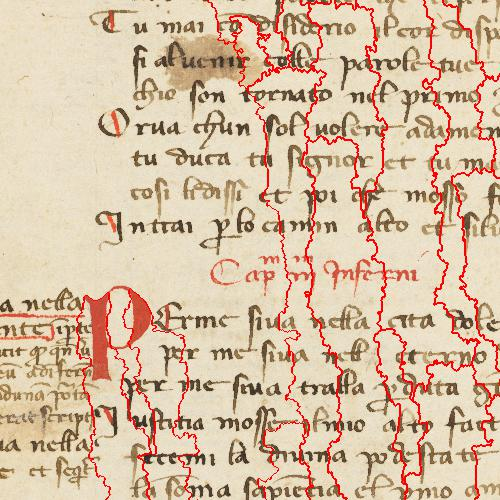
\includegraphics[width=0.24\textwidth]{figures/img/mark_boundaries_m0.jpg}
    }
    \subfloat[\(m = 1\)]{
        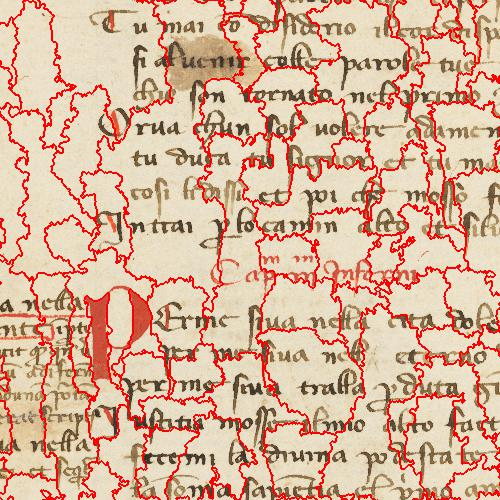
\includegraphics[width=0.24\textwidth]{figures/img/mark_boundaries_m1.jpg}
    }
    \subfloat[\(m = 10\)]{
        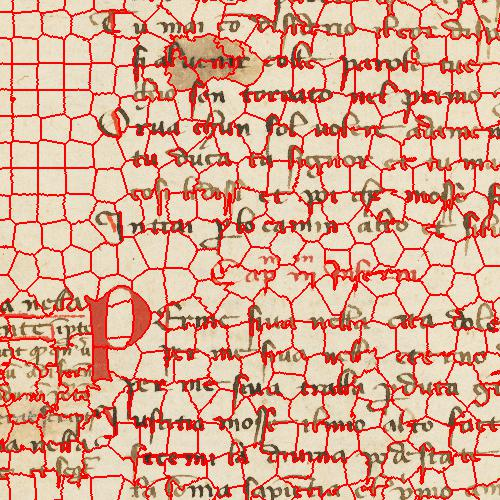
\includegraphics[width=0.24\textwidth]{figures/img/mark_boundaries_m10.jpg}
    }
    \subfloat[\(m = 100\)]{
        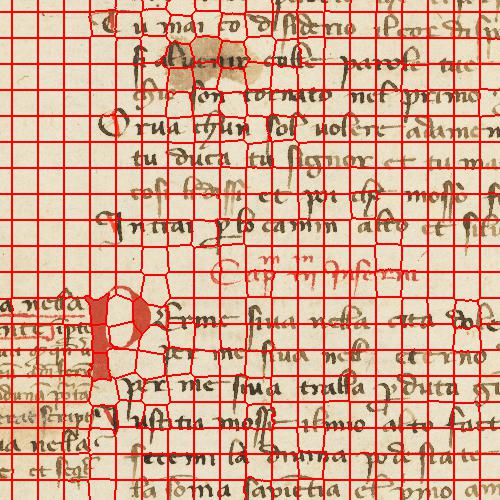
\includegraphics[width=0.24\textwidth]{figures/img/mark_boundaries_m100.jpg}
    }
\end{figure}

\citeauthor{AchantaSLICSuperpixelsCompared2012} stellen später zwei wichtige Erweiterungen vor:
Normalisierung des Distanzmaßes und Adaptive-SLIC.

\citeauthor{ChenConvolutionalNeuralNetworks2017a} nennen keine Details zur Wahl
der Superpixel-Parameter, verweisen aber auf eine frühere Studie die sich mit unterschiedlichen 
Superpixel verfahren beschäftigt \parencite{ChenPageSegmentationHistorical2016}.
Die Studie versucht einen Autoencoder (siehe \ref{sec:autoencoder}) zu trainieren auf Basis von Superpixeln und vergleicht dabei den Einfluss von unterschiedlichen Superpixel-Methoden. Die veröffenlichen Ergebniss zeigen aber nur die Performanz im Bezug
auf die Zahl der Cluster \(n \in \left\{10^3, 50^3, 100^3, 200^3\right\}\) und dem Skalierungsfaktor \(\alpha \in \left\{2^{-2}, 2^{-3}\right\}\)
\qq{adaptive slic}
\qq{Problem gt zu treffen}

\section{Netzwerk-Architektur}
\citeauthor{ChenConvolutionalNeuralNetworks2017a} beschreiben die Struktur
des CNN als \(28 \times 28 \times 1 - 26 \times 26 \times 4 - 100 - M\).

Während des Trainings wird das Ground-truth Label des Zentrumpixels als Label für den Superpixel verwendet.

\section{Training}

\section{Nachverarbeitung}
\section{\textcite{XuPageSegmentationHistorical2017}}
Das Paper \citetitle*{XuPageSegmentationHistorical2017} von \citeauthor*{XuPageSegmentationHistorical2017} verfolgt einen anderen Ansatz.
\citeauthor{XuPageSegmentationHistorical2017} verwenden eine Netwerk  


\section{VGG}


\section{Deconvolution}

\section{Ergebnisse}